% latexmk -pvc -pdf
\documentclass[9pt, a4paper]{article}
\usepackage[margin=0.65in]{geometry}
\usepackage{graphicx}
\usepackage{caption}
\usepackage{amsmath,amsthm,amsfonts,amssymb}
\usepackage{blindtext}
\usepackage[english]{babel}
\newenvironment{Figure}
    {\par\medskip\noindent\minipage{\linewidth}}
    {\endminipage\par\medskip}

% \newcommand\II{\mathbb{}}
% \newcommand\PT{\textit{}}

\title{Simulating phase contrast imaging for materials with variable density}
\author{Ana C. Fabela Hinojosa \\
\small{Supervisors: Prof. Marcus Kitchen}}
\small{\date{\today,  \\Due date: Friday 26\textsuperscript{th} August, 2021}}

\begin{document}
\maketitle
\section{Current objective}
In this project I study the theoretical perspective of of coherent X-ray imaging. My current focus is to investigate via a simulation how the phase of incident X-rays changes as the density of a material in an arbitrary imaging system changes. My investigation will be extended by simulating two distinct materials under the same wave-field and see if and how distinctly phase contrast occurs. The eventual goal of this simulation is to verify if successful phase retrieval can be done of the imaged objects given their variable densities.

\section{The fundamentals of X-ray imaging theory}
The mathematical background of the field of X-ray optics lies with the Maxwell equations of electromagnetism\cite{PagsTutes}. Maxwell's equations describe electromagnetic field disturbances as waves moving at a now well known speed \textit{c}. From revolutionary contribution of Maxwell's equations to mathematical physics it is clear that any electromagnetic wave-field can be studied using the wave equation.

\subsubsection{Helmholtz equation and the Angular spectrum formulation}
The Helmholtz equation represents a time-independent form of the wave equation and it is a central equation of diffraction theory\cite{CH49}\cite{Pags2006}\cite{Helmholtz}.
In general, radiological imaging is done with polychromatic X-rays with non-trivial spectra\cite{CH49}. It is possible to use spectral decomposition of the wave function into monochromatic components and therefore simplify the imaging process greatly. The separation of each component with an individual fixed angular frequency (i.e. a trivial dependence in time), transforms the wave equation into a time-independent partial differential equation (PDE) that is applied individually to each monochromatic component. After the analysis of each component is done, a recombination of the monochromatic components results in the complete description of the polychromatic process\cite{CH49}\cite{Pags2006}. This method is known as the \textit{angular spectrum formulation}. 
% Here I present a derivation of the Helmholtz equation

The complex scalar wave-field function $\Psi(\vec{r},t) = \sqrt{I(\vec{r},t)} \mathrm{exp}(i \phi(\vec{r},t))$ obeys the wave equation in a vacuum
\begin{equation}\label{eq:1}
\left ( \frac{1}{c^2} \frac{\partial^2 }{\partial t^2} -\nabla^2 \right ) \Psi(\vec{r},t) = 0,
\end{equation} 
where \textit{c} is the speed of light and $\nabla$ is the Laplacian operator.
The spectral decomposition of $\Psi(\vec{r},t)$ is done via the Fourier transform
\begin{equation}\label{eq:2}
\Psi(\vec{r},t) = \frac{1}{\sqrt{2 \pi}} \int_{0}^{\infty}\psi_{\omega}(\vec{r}) e^{-i\omega t}d\omega,
\end{equation}
notice that the integral only considers a positive integration range (due to analyticity concerns\cite{PagsTutes}). In this equation the spatial wave-function subscript $\omega$ indicates functional dependence on this quantity\cite{Pags2006}. Evaluating equation (\ref{eq:1}) using equation (\ref{eq:2}) yields the Helmholtz equation for the vacuum
% \begin{equation}\label{eq:3}
% \left ( \frac{1}{c^2}\frac{\partial^2}{\partial t^{2}} - \nabla^{2}  \right )\Psi(\vec{r},t) = 0,
% \end{equation}
% \begin{equation}\label{eq:4}
% \therefore \int_{0}^{\infty} \frac{1}{\sqrt{2 \pi}} \left ( \frac{1}{c^2}\frac{\partial^2}{\partial t^{2}} -\nabla^{2}  \right )  
% \psi_{\omega}(\vec{r}) e^{-i\omega t}d\omega = 0,
% \end{equation}
% \begin{equation}\label{eq:5}
% \therefore \int_{0}^{\infty} \frac{1}{\sqrt{2 \pi}} \left ( \frac{-\omega^2}{c^2}\psi_{\omega}(\vec{r}) e^{-i\omega t} -\nabla^{2}\psi_{\omega}(\vec{r}) e^{-i\omega t} \right ) d\omega  
%  = 0,
% \end{equation}
\begin{equation}\label{eq:6}
\left ( k^2 + \nabla^{2} \right ) \psi_{\omega}(\vec{r})  
 = 0,
\end{equation}
where the wave vector $k = \omega/c$.

\subsubsection{Paraxial fields}
In most situations involving phase-contrast imaging, X-ray fields behave as paraxial fields. Electromagnetic energy in this context is concentrated within a small region about the beam axis. A beam is an EM wave propagating in free space with small divergence (i.e. spread) away from the propagation axis, hence the origin of the name \textit{paraxial}.

In the previous section I described $\Psi(\vec{r},t)$ as a complex scalar wave-field, I will now add to this description the paraxiality condition.
Under this approximation the complex disturbance $\psi_{\omega}(\vec{r})$ present in the Helmholtz equation is expressed as a product of a z-directed plane wave and a perturbing envelope\cite{PagsTutes}\cite{CH49}
\begin{equation}\label{eq:7}
\psi_{\omega}(\vec{r}) = \Phi(\vec{r})\mathrm{exp}(ikz),
\end{equation}

 \begin{Figure}
 \centering
 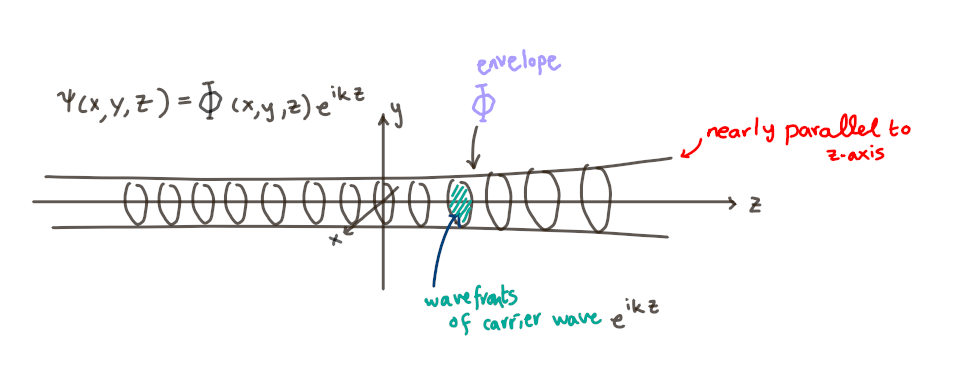
\includegraphics[width=0.6\linewidth]{paraxial_beam.png}
 \captionof{figure}{cartoon of a paraxial wave-field $\psi_{\omega}(\vec{r})$ displaying beam propagation properties along the z-axis. The slowly varying complex envelope is modulated by a carrying plane wave.}
\end{Figure}
Note that the longitudinal variation of the complex envelope $\Delta z = \lambda = 2 \pi/k$ is required to be smaller than the complex envelope itself
\begin{equation}\label{eq:8}
\frac{\Delta \Phi(\vec{r})}{\Phi(\vec{r})} \leq 1
\end{equation}
using equation (\ref{eq:8}) and the longitudinal variation $\Delta z$  in the Helmholtz equation yields the paraxial Helmholtz equation in the vacuum
\begin{equation}\label{eq:9}
\left (\nabla_{T}^{2} + 2 i k \frac{\partial }{\partial z}\right ) \Phi(\vec{x , y, z}) = 0
\end{equation}

\subsubsection{Refractive index and the projection approximation}
In the presence of static, non-magnetic, scattering material media the complex scalar X-ray wave-field can still be studied by using the inhomogeneous Helmholtz equation 
\begin{equation}\label{eq:10}
\left ( k^2 n^2 (\vec{r}) + \nabla^{2}  \right )\Psi(\vec{r},t) = 0,
\end{equation}
where $n(\vec{r})$ is the position dependent and complex form for the refractive index, the real part of which corresponds to the refractive index and the imaginary part of this complexified refractive index can be related to the absorptive properties of a sample\cite{PagsTutes}.
\begin{equation}\label{eq:11}
n = 1 - \delta + i \beta,
\end{equation}
where $|\delta|, |\beta| << 1$. Using the complex refractive index in the inhomogeneous paraxial Helmholtz equation yields the \textit{projection approximation}, which is an expression that describes the phase shift and attenuation undergone by an X-ray wave moving across a sample
\begin{equation}\label{eq:12}
\Phi(x, y, z_0) = \mathrm{exp} \left ( -ik \int_{0}^{z_0}(\delta - i\beta)dz\right ) \Phi(x, y, 0)
\end{equation}

 \begin{Figure}
 \centering
 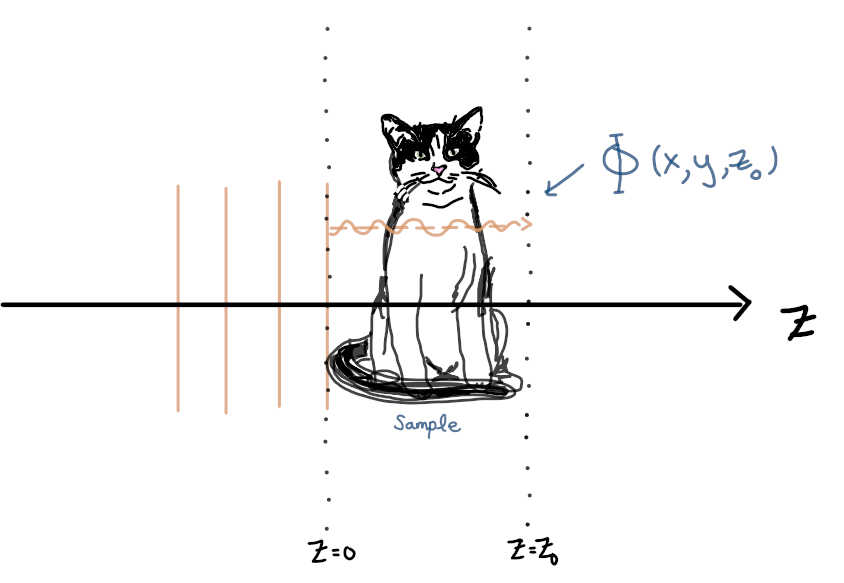
\includegraphics[width=0.6\linewidth]{projection_approximation.png}
 \captionof{figure}{Schematic diagram of the projection approximation adapted from references \cite{CH49} and \cite{Pags2006}. The sample and is contained within the space between $z = 0$ and $z = z_0$. The sample is described by its refractive index $n(\vec{r})$ which differs from the the refractive index of the air volume that surrounds the sample.In this figure one can see that the path of X-rays passing through an object can be described by defining a surface immediately downstream from the irradiated object (i.e. $z = z_0$) at which the transferred transverse intensity and phase changes of the incident X-rays are imprinted\cite{CH49}. }
\end{Figure}

The projection approximation assumes that X-ray flow may be well approximated by straight lines parallel to z\cite{PagsTutes} and that most X-rays passing through an object do not actually interact with the sample material (i.e. minimal scattering occurs within the sample, a fair assumption due to small magnitude of the complex \textit{refractive index}). Neglecting scattering effects is mathematically equivalent to discarding the transverse Laplacian term in equation (\ref{eq:9})\cite{CH49}, in addition terms corresponding to the X-ray--matter interaction must be added to equation (\ref{eq:9}) making it the inhomogeneous paraxial Helmholtz equation
\begin{equation}\label{eq:13}
\left ( 2 i \frac{\partial }{\partial z} + k ( n^2 (x, y, z) - 1 )\right ) \Phi(\vec{x , y, z}) = 0.
\end{equation}


% \subsubsection{Phase shift}

% Phase-contrast yields a quantity that is related to the real part, $\delta$\cite{CH49}.

% phase-contrast methods enable tiny differences in the real part of the refractive index to be more readily measured over attenuation contrast. In other words, phase-contrast may offer an advantage when one needs to distinguish between different types of soft tissues (Pelliccia et al. 974).

% \subsubsection{Transport of intensity equation}

% \begin{equation}
% \left ( \frac{1}{c^2} \frac{\partial^2 }{\partial t^2} -\nabla^2 \right )\mathbf{E}(\vec{r},t) = 0,
% \end{equation} 

% \begin{equation}
% \left ( \frac{1}{c^2} \frac{\partial^2 }{\partial t^2} -\nabla^2 \right )\mathbf{B}(\vec{r},t) = 0.
% \end{equation} 


% \section{Investigations}

% \subsubsection{}


% \subsubsection{}


% \section{Future Plans}


% \section{Conclusion}


\bibliography{mybib}
\bibliographystyle{unsrt}
\end{document}

